% Allow relative paths in included subfiles that are compiled separately
% See https://tex.stackexchange.com/questions/153312/
\providecommand{\main}{..}
\documentclass[\main/thesis.tex]{subfiles}

\begin{document}

\chapter{Introduction}

%% TODO
 % AH: Tell us you want to generate synthesizers and the benefits of code over 1000s of NN parameters.
 
\section{What is Our Goal?}
Novel, one-shot\footnote{A single hit on the drum that captures its capabilities} drum sounds are not easy or cheap to find. New drum sounds can be obtained via live recordings of drums, layering existing drum sounds or creative (often lengthy) hacking of sound engineering techniques. Our goal here is to create a new, virtual source of novel drum sounds, which could then be used in electronic music compositions.

\section{Why Does the World Need More Drums?}
 Percussive sounds are often created by striking of a percussive instruments. Percussive noise is often used for creation of rhythm in a composition~\cite{needham1967percussion}. Drum sounds such as kick and snare are two of the most common examples of percussive sounds~\cite{barry2005drum}. In this work we are looking for sounds which can be used as substitutes for drums in experimental and eclectic compositions and are not concerned with the nuances of drum vs percussive sounds. As a result, we often use "drum" and "percussion" interchangeably.

 Drum sounds are used frequently by music artists. A common approach to creation of drum tracks for digital music is to combine short recordings of real-life drums and other percussive elements in order to create a new drum-kit. This approach frees artists from the need to obtain and store real life instruments while enabling endless combinatorial possibilities. However, by relying on recordings of \textit{real life} drum sounds, we are still limited by what drums exist in the real world and whether or not we have access to clean, one-shot recordings. Our hypothesis is that the virtualization of sound generation can alleviate these material limitations. 
 
\section{What Solution Do We Propose?}
To virtually create novel drum sounds, we need a generative source; One that produces audio based on some instructions. We also need a method of evaluation to help us determine which sounds resemble drums and are worth keeping. We also would like to know what instructions caused our audio source to make the sounds we liked. In short, our approach requires effective \textit{generation} and \textit{evaluation} of sounds. 

\section{What Tools Are at Our Disposal?}
\label{sec_tools_disposal}
We can conceptualize utilizing digital sound synthesis in various ways. An ideal scenario would be a graphical, 3D simulation of virtual drums; Where we could modulate the thickness, dimensions and material of the frame, the drum skin, the type of impact, etc. before rendering the sound of the simulation. Unfortunately, such 3D systems are not yet practical \cite{langlois2016toward}. State of the art generative networks utilized in works by Ramires et al. \cite{ramires2020neural} and Aouameur et al.\cite{aouameur2019neural} 
are another promising avenue; However, for reasons such as efficiency, tractability and novelty (discussed further in related works \ref{related}), we strive towards more tractable methods that utilize simple, tried and true signal generation tools in tandem with machine learning techniques to rapidly generate new sounds and evaluate their desirability.

Before we further cover details of the project, it's important to give a quick introduction to the basics of computerized audio generation and evaluation that were made use of in this project.
\subsection{How Can A Computer Make Sounds?}
\ref{sec:computer makes sound}
Your computer can make a wide variety of sounds in wide variety of ways. You can use it to record real life audio and play it back. You can hit its various instruments, surfaces, and objects with a drumstick. You can also program it to make noise using software.
Sounds are transmitted via waveforms. Your computer can emulate the physical characteristics of basic waveforms by evaluating the output of periodic functions such as sines and cosines. Evaluation of basic periodic functions is the simplest form of software audio generation \cite[chapter~5]{mitchell2009basicsynth}.

For example, think of the universally recognizable "dialing" sounds (DTMF) that communication networks use during typical phone calls. You can program your computer to make similar noises by feeding a range of equally spaced values between 0 and $2\pi$ to a sinusoidal function at a rate that's audible to human ears\footnote{Human audible range is approximately 30Hz to 15000KHz}. 

This generative system is called an \textit{oscillator} and its output is a waveform which can be sent to your computer's digital-to-analog conversion system to create an audible signal. The combination and modification of these pure tones are the building blocks of digital signal processing (DSP).

% inspired by chapter 5 graph of mitchell (waiting adaption permission(granted)
\begin{figure*}[h]
\label{fig_example_sine}
\centering
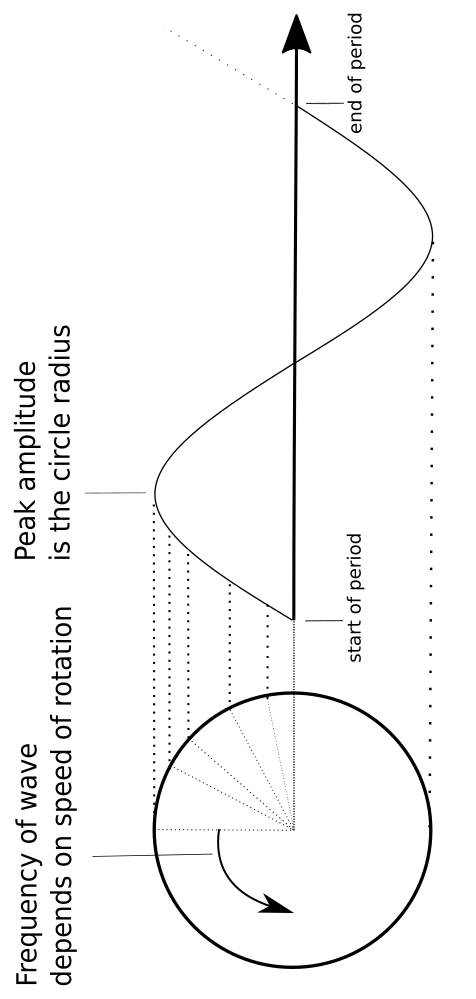
\includegraphics[width=0.45\linewidth,angle =-90 ]{images/periodic_function.png}
\caption{A computer can simulate waveforms by utilizing periodic functions. Digital waveforms are discrete approximations of analogue waves. \cite{mitchell2009basicsynthChap5} }
\end{figure*}


 Most organic sounds---sounds from the natural environment, and its flora and fauna---are much more complex than the output of a single oscillator and their digital approximation requires a combination of multiple (perhaps thousands) of pure tones. However, with careful programming, DSP techniques can be used to replicate almost any sound, which is why they have powered commercial digital synthesizers for over half a century \cite{jenkins2019analog} and continue to remain a popular method of audio synthesis amongst artists. Another advantage to using DSP for sound generation is that the synthesizers we build using these functions are tractable: the output is determined by the input and reproducible. This makes the evaluation of a set of inputs (or parameters) to our synthesizers  simpler compared to the evaluation of synthesizers that utilize probabilistic models.
 
In the next chapters we will discuss our work towards a system for automatic \textit{generation of sounds}, capable of rapid generation of short (under 1 second) audio clips. Our approach entailed the implementation of a virtual sound synthesizer that can take a set of instructions, or \textit{programs}, as input and generate the corresponding audio. A by-product of this approach is that the sounds generated may sound extremely in-organic, yet perfectly usable by more experimental artists, adding a desirable "novel" factor. 



\subsection{How Can a Computer Evaluate Sounds?}
Automatic evaluation of sounds is an essential component of our work: A thorough manual evaluation of outputs is not possible when hundreds can be created in a second. How can a computer help us evaluate sounds?

Suppose a person is given a set of recordings of solo musical instruments being played by various skill levels and asked to categorize them however they please. There is a long list of features that the person could use: the length of audio recordings, the skill of the player, the timbre of the instrument (which is related to the type of instrument: wind, string, percussion etc.) the rhythm and so on. 

 Computers can be programmed to quickly extract the majority of these feature types for us. With shorter audio clips (such as the drum sounds we're interested in), personal subjectivity might play a smaller role in describing sounds, making the categorization task easier.

In our work, we find simple features such as frequency content (high pitch vs low pitch), length, and envelope (change in loudness, how fast the sounds reaches its maximum loudness and fades away) to be powerful features for the categorization of drum sounds. Later on we will discuss our algorithms for extraction of these and other features in \ref{impl}. We will also discuss how these extracted features were used to train models that can automatically categorize new sounds.  
%  We will cover our curation of a database of sounds \ref{data} and its usage for the design and training of machine learning models to learn the characteristics of different drum groups. We will discuss how these models can be used rapidly evaluate each output and curate those which resemble drum sounds.

%% TODO: Throw a diagram in here?
\section{What Is Our Methodology?}
\label{sec_methodology}
Given the tools at our disposal, our attempt is centered around a generative pipeline of audio. The outputs of this pipeline are evaluated and the evaluation score is used to further improve the pipeline and separate undesired outputs from desired ones. We want random sounds to be created by a tractable source, we also want to evaluate these sounds so we can guide the random sound generator towards desired sounds. Instead of learning weights and parameters in an audio-generation neural network, we wish to generate, search, and tune synthesizers to produce percussion sounds. Following this idea, we found the proper implementation of 2 major components to be crucial:

\begin{itemize}
    \item \textit{Virtual Synthesizer}: A flexible, deter\-min\-istic, and tract\-able gener\-ator which can create audio. 
    \item \textit{Virtual Ear}: An ear that returns an evaluation of an audio sample; estimating the effectiveness of an audio sample's fulfillment of a producers requirements. The ear's evaluation guides the generation process towards a desired path, making it a crucial component of our pipeline. 
\end{itemize}
% AH: Optional. Can be removed or reduced later
Our components are designed with modularity and parallelizability in mind. This allows each component to be debugged, modified, and improved without requiring modifications in other components while additionally increasing the scalability and speed of experiments. 
Section \ref{impl} contains further discussion of the components as well as the code that glues the project together.

While the main focus of this project is the generation of novel percussive sounds, our methodology indicates promising results with regards to creation of new presets for any virtual synth without the need for a-priori knowledge of the functions or its parameters (i.e the effect of parameter modulation on the sonic output). We also demonstrate the viability of a virtual synthesizers based on Digital Signal Processing (DSP) methods for fast, unsupervised creation of novel audio, discussed in more detail in section \ref{related}. 


\section{Restating the Goal}
We want to leverage AI technologies, such as heuristic search and random search, to produce new drum samples, by finding synthesizers and their appropriate configurations that can produce various kinds of drum samples. Effectively we will combine machine listening and code generation of synthesizers to find drum samples.

Our work is motivated by the idea of finding new, convenient methods for the expansion of a music producer's library of sounds. Primarily with generation of novel, one-shot audio samples but also with automated search and creation of presets for virtual synthesizers. Using the generation of short, percussive audio samples as a starting point, this project is a proof of concept for a promising avenue towards our motivational goal.


\end{document}